% In part I of this book, we investigated transmission lines and their properties, and electromagnetic waves and their propagation in the unbound and semi-bound medium. We investigated specifically the reflection and refraction of an electromagnetic wave in a dielectric boundary. We saw the reflection of electromagnetic waves from the conducting boundary.

% So in part II of the book, we will further bound the medium of propagation of the waves (introduce waveguide structures), explore the parallel plane, rectangular and circular waveguides and the modes of propagation that can be excited in these structures. Then, we will explore the basics of antenna theory and look at concepts like radiation, radiation patterns, receiving antennas, and antenna arrays.

\chapter{Parallel plane waveguides (1)}\label{lec:lec35}
Having laid the foundation of electromagnetic wave propagation in an unbound or semi-bound medium and the reflection and refraction of these waves in a dielectric boundary, we are prepared to discuss to some level granularity waveguide structures. We will start with the simplest waveguide structure which is the parallel plane waveguide. We will then move on to the rectangular waveguide and then the circular waveguide. We will also discuss the modes of propagation that can be excited in these structures.

\section{Waveguide}\index{Waveguide}
A \textit{waveguide} is a guiding structure capable of efficiently transmitting electromagnetic energy from one point to another. While coaxial cables and parallel wire transmission lines do exhibit waveguiding characteristics, they suffer from significant losses at higher frequencies, making them less suitable for efficient transmission in such regimes. Consequently, at frequencies in the GHz and tens of GHz range, hollow-pipe waveguides with rectangular or circular cross-sections become more prevalent. These waveguides offer improved transmission efficiency and reduced losses, making them highly suitable for high-frequency applications, including microwave communication, radar systems, and various wireless technologies.

Indeed, waveguides play crucial roles in communication engineering, especially when dealing with high frequencies. In communication systems, the goal is to find waveguide structures that can efficiently transfer energy from one point to another while minimizing losses. To achieve this, the waveguide structures should possess certain characteristics:

\begin{enumerate}[(i)]
\item They should be compact and small in size to facilitate ease of transport and installation.
\item They should be malleable, allowing them to be moulded into desired sizes and shapes to suit specific communication needs.
\end{enumerate}

To understand the behaviour of such waveguide structures, we typically start by employing Maxwell's equations and imposing appropriate boundary conditions to obtain solutions for particular problems. However, in this exploration, we will take a different approach. We will examine if, by adhering to the uniform plane wave boundary conditions, we can deduce the behaviour of a waveguide-like structure. Specifically, we will focus on the \emph{Parallel Plane Waveguide}.

As the name suggests, this waveguide comprises two parallel planes separated by a finite distance. Electromagnetic energy becomes confined between these planes, allowing it to propagate along the structure, effectively trapped within this waveguide.

\section{Parallel Plane Waveguide}\index{parallel plane waveguide}
In Part I, we explored the reflection of wave propagation from a conducting boundary. Specifically, we considered a conducting boundary upon which an incident wave impinges at an angle $\theta$, as illustrated in Figure~\ref{fig:lec35fig1}. The reflected wave emerges from the boundary at an angle $\theta$ with respect to the normal.

By imposing appropriate boundary conditions, we derived the reflection coefficient for the electric field, which was found to be $-1$. This implies that the conducting boundary behaved equivalently to a short circuit in a transmission line. The reflection coefficient indicates that the magnitude of the reflected electric field is equal to the magnitude of the incident electric field but with a phase change of 180\textdegree.
\begin{figure}[h]
\centering
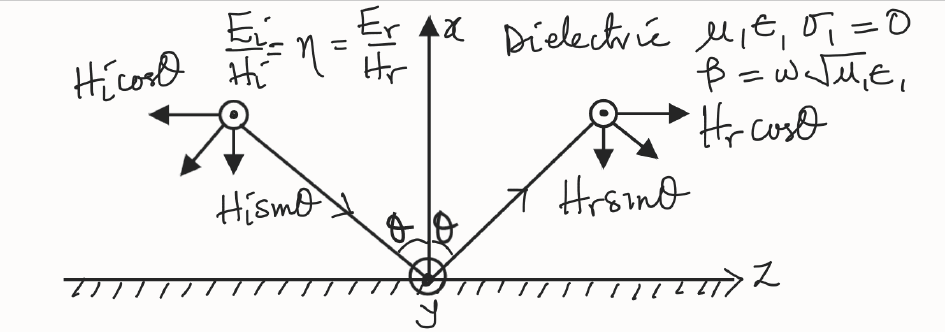
\includegraphics[width=1\linewidth]{\pathtoparttwo/graphics/lec35fig1}
\caption{Incident and reflected electromagnetic wave on a conducting boundary}
\label{fig:lec35fig1}
\end{figure}

We observed that the electric field $\bar{E}$ in the medium is a superposition of the incident and reflected fields. The electric field can be expressed as $\bar{E} = \jmath 2E_i\sin(\beta x\cos\theta)e^{-\jmath\beta z\sin\theta}$, where $\beta$ is the phase constant, $\theta$ is the angle of incidence, and $E_i$ represents the incident electric field amplitude. The magnetic field $H$ consists of standing and travelling waves.

We can exploit the behaviour of the electric field to create a guiding structure for electromagnetic energy. By trapping energy from both sides of a semi-infinite dielectric medium, we can create a parallel plane waveguide. The tangential component of the electric field at the interface ($x=0$) should be continuous. However, we observed that at certain distances $x=\frac{m\lambda}{2\cos\theta}$ (where $\lambda$ is the wavelength), the electric field becomes zero. Placing a conducting sheet tangential to the electric field at these points does not alter the boundary conditions.

Consequently, for different values of $m$ (where $m=0, 1, 2, 3, \ldots$), we can insert conducting sheets at $x=\frac{m\lambda}{2\cos\theta}$ without affecting the electric or magnetic field distributions. The field distribution remains unchanged when these boundaries are introduced at the specified points, as illustrated in Figure~\ref{fig:lec35fig2}, which displays the variation of $E_y$, $H_x$, and $H_z$ with $x$.

The parallel plane waveguide is a result of this arrangement, where electromagnetic energy is guided and propagated between two parallel conducting sheets without being trapped. The points where the conducting sheets can be inserted without disturbing the field distribution are vital for defining the guiding structure and ensuring efficient wave propagation within the waveguide.
\begin{figure}[h]
\centering
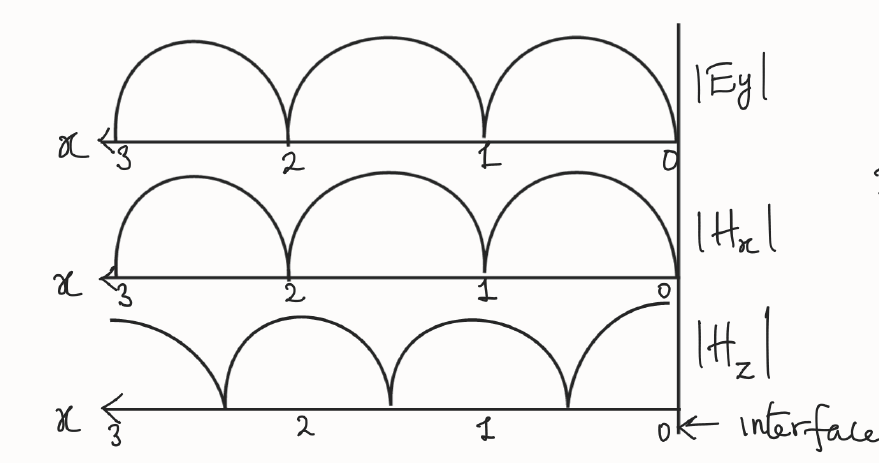
\includegraphics[width=1\linewidth]{\pathtoparttwo/graphics/lec35fig2}
\caption{Variations of components of electric and magnetic fields}
\label{fig:lec35fig2}
\end{figure}

Indeed, inserting a conducting sheet at position 1 in Figure~\ref{fig:lec35fig2} above the interface leads to the trapping of the electromagnetic wave between two boundaries. The wave becomes confined within a closed structure, transforming the originally semi-infinite medium into a bounded one in the x-direction. The conducting planes can also be placed at positions 2, 3, and so on, resulting in electromagnetic energy being trapped between these parallel planes with a separation of phases given by $x=\frac{m\lambda}{2\cos\theta}$.

The resulting waveguide structure is depicted in Figure~\ref{fig:lec35fig3}. In this configuration, the reflected electric field has the same magnitude as the incident field but propagates into the plane (i.e., into the paper) contrary to the direction of the symbol used for $H$. The electromagnetic fields within this waveguide structure are described by three components: the electric field ($E$) is oriented in the $\hat{y}$ direction, while the magnetic field ($H$) has components in the $\hat{x}$ and $\hat{z}$ directions, lying in the $\hat{x}\hat{z}$ planes.

The electric field is perpendicularly polarized and tangentially oriented to the plane of incidence. At a distance of $\frac{\lambda}{2\cos\theta}$ above the interface, the tangential component of the electric field becomes zero. Similarly, at twice this distance, $2\left(\frac{\lambda}{2\cos\theta}\right)$, from the interface, the tangential component of the electric field is zero again. Consequently, a conducting sheet can be placed at any of these distances above the interface plane without altering the field distribution.

By introducing a conducting plane at $x=\frac{\lambda}{2\cos\theta}$, the electromagnetic wave propagates only within the bounded region. The wave undergoes multiple reflections between the two conducting interfaces, leading to the wave travelling along the waveguide structure or planes. These multiple reflections allow the wave to be guided and confined within the boundaries, enabling the propagation of electromagnetic energy along the structure.
\begin{figure}[h]
\centering
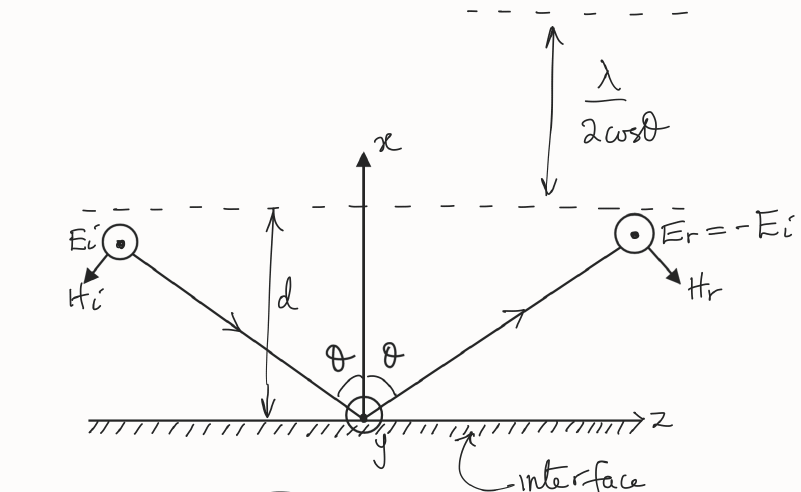
\includegraphics[width=1\linewidth]{\pathtoparttwo/graphics/lec35fig3}
\caption{Incident and reflected electromagnetic wave on a conducting boundary showing the distances when the electric field goes to zero}
\label{fig:lec35fig3}
\end{figure}

Let us invert the problem, i.e. \emph{knowing the angle $\theta$, what will be the separation of these planes so that the electric field will not be affected?} This is what we have just done. Similarly, \emph{given a separation of these two conducting planes as $d$, what angle should the electromagnetic wave be launched such that it can propagate along z or its propagation will be sustained?} 
\begin{align*}
d =& \frac{m\lambda}{2\cos\theta}\\
\cos\theta =& \frac{m\lambda}{2d}\quad\text{$m$ is a discrete number $1, 2, 3, \ldots$.}
\end{align*}
This equation provides us with the required launch angle $\theta$ for a given separation $d$ between the conducting planes, such that the electromagnetic wave can propagate along the z-direction and sustain its propagation within the waveguide.

However, it is important to note that for a given value of $d$, the angle $\theta$ is not continuous. Only specific discrete angles will allow the sustained propagation of the electromagnetic wave along the structure. This constraint on the launch angle is different from the behaviour observed in unbounded media, where there were no restrictions on the launch angle. Similarly, in the case of a semi-finite medium (dielectric of the conductor), we could have any angle of incidence and observed semi-field distribution.

In the waveguide structure with two conducting planes, the discrete values of $m$ and the corresponding angles $\theta$ define the set of angles at which the electromagnetic wave can propagate efficiently and sustain its propagation along the z-direction. These discrete launch angles are crucial for guiding the electromagnetic energy within the waveguide and ensuring efficient transmission and propagation of the wave.

\section{Modal Propagation}\index{modal propagation}
In the case of bound structures, such as the parallel plane waveguide, electromagnetic waves cannot be launched at arbitrary angles of incidence. Waves launched at angles that do not satisfy the condition $\cos\theta = \frac{m\lambda}{2d}$ will be rejected by the structure and will not propagate within it. Only when the wave is launched at discrete angles, corresponding to specific values of $m$, will there be sustained propagation. This phenomenon is known as \textit{Modal Propagation}.

For each value of $m$, there is a unique pattern of electric and magnetic fields created within the bound structure. The patterns for $m=0$, $m=1$, $m=2$, and so on, are distinct from each other. Thus, we have discrete electric and magnetic field patterns that can survive inside the bounded structure, and this characteristic of wave propagation is termed \textit{Modal Pattern}\index{modal pattern}. Modal propagation is fundamental to all waveguiding structures, including parallel plane waveguides, rectangular waveguides, and fibre optics. It defines how electromagnetic energy travels in definite patterns within these structures.

Notably, the range of possible $\theta$ is constrained to values between 0 and 1, as $0 \leq \cos\theta \leq 1$. Additionally, for a given separation $d$ between the conducting planes, the number of discrete angles (corresponding to different values of $m$) at which the wave can be launched is limited. Once $\frac{m\lambda}{2d}$ becomes greater than 1, the corresponding angles are no longer physical angles $\theta$. Therefore, there are a finite number of uniform plane waves that can be launched in the given space between the boundaries until $\frac{m\lambda}{2d} > 1$.

In a parallel plane waveguide with two boundaries, the notion of incident and reflected waves changes. As one wave is incident on one boundary, it becomes a reflected wave when it reaches the opposite boundary, and vice versa. In this scenario, wave propagation can be visualized as two sets of waves travelling in opposite directions, from the top plane to the bottom plane and vice versa. The superposition of these two sets of waves creates a field distribution inside the bound structure, leading to the emergence of the modal pattern. The modal pattern is illustrated in Figure~\ref{fig:lec35fig4}, where the propagation of the electromagnetic wave is represented as the superposition of two waves travelling at an angle with respect to the boundary or perpendicular to the boundary.

With this understanding, finding out the electric and magnetic fields becomes straightforward. So we make some conclusions on the basis of the above discussion:
\begin{enumerate}[(i)]
\item Wave survives at discrete angles in a parallel plane waveguide and,
\item These discrete angles are a finite number of angles at which the wave survives
\end{enumerate}
\begin{figure}[h]
\centering
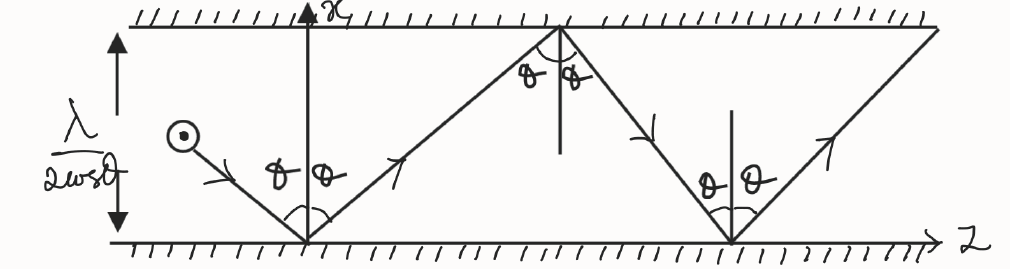
\includegraphics[width=1\linewidth]{\pathtoparttwo/graphics/lec35fig4}
\caption{Wave propagation in a medium of two parallel conducting boundaries}
\label{fig:lec35fig4}
\end{figure}

We observed that in Figure~\ref{fig:lec35fig4} multiple reflections are occurring between the two conducting boundaries. As a result, the net propagation of energy is in the z-direction (see Figure~\ref{fig:lec35fig5}), parallel to the axis of the waveguide. The electric field, $E$, is oriented perpendicular to the plane of incidence, which in this case is the plane of the paper. Thus, during reflection, the electric field vector remains perpendicular to the plane of incidence.

On the other hand, the magnetic field ($H$) direction changes from one point to another, as depicted in Figure~\ref{fig:lec35fig4}. The figure shows the directions of the incident magnetic field, $H_i$, and the reflected magnetic field, $H_r$, while the incident and reflected electric fields, $E_i$ and $E_r$, respectively remain oriented in the $\hat{y}$ direction.
\begin{figure}[h]
\centering
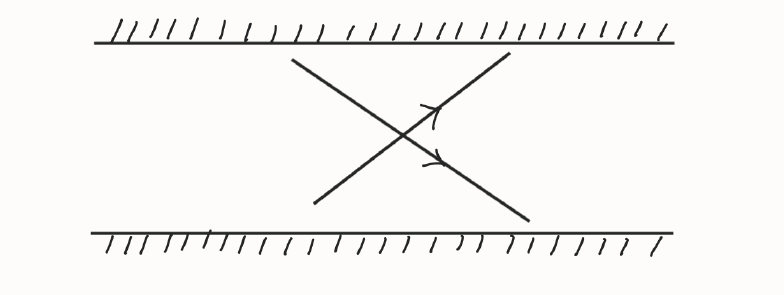
\includegraphics[width=1\linewidth]{\pathtoparttwo/graphics/lec35fig5}
\caption{Wave propagation in a medium of two parallel conducting boundaries showing the superposition of waves}
\label{fig:lec35fig5}
\end{figure}

So $H_i$ and $H_r$ keep changing direction, and the magnetic field inside the plane waveguide has two components, x and z components respectively. Since the net propagation is in the z direction, the magnetic field essentially has components in the direction of net propagation components perpendicular to the direction of net propagation.

From Equations~\eqref{en:totalelectricfield2},~\eqref{eqn:totalmagfieldx3} and~\eqref{eqn:totalmagfieldz2}, we can rewrite the components of the electric and magnetic field with $\cos\theta$ substituted with $\frac{m\pi x}{d}$ and $\sin\theta = \sqrt{1 - \cos^2\theta}$ as follows:
\begin{dmath}
E=\jmath 2 E_i \sin(\frac{m\pi x}{d})\footnotemark e^{-j\beta z\sqrt{1 - \left(\frac{m\lambda}{2d}\right)^2}} \hat{y}
\label{eqn:totalelectricfield3}
\end{dmath}
\footnotetext{
Since, $\beta = \frac{2\pi}{\lambda}$, then $\beta\cos\theta = \beta\times\frac{m\lambda}{2d} = \frac{2\pi}{\lambda}\times\frac{m\lambda}{2d}=\frac{m\pi}{d}$
}
\begin{dmath}
H_x = -\jmath 2\frac{E_i}{\eta}\sin\theta\sin(\frac{m\pi x}{d}) e^{-\jmath 2\beta z\sqrt{1 - \left(\frac{m\lambda}{2d}\right)^2}}
\label{eqn:totalmagfieldx4}
\end{dmath}
\begin{dmath}
H_z = -\frac{2E_i}{\eta}\left(\frac{m\lambda}{2d}\right)\cos(\frac{m\pi x}{d})e^{-\jmath 2\beta z\sqrt{1 - \left(\frac{m\lambda}{2d}\right)^2}}
\label{eqn:totalmagfieldz3}
\end{dmath}
These are the three fields which can survive in a particular waveguide for a perpendicularly polarized electric field (perpendicular to the plane of incidence). Now the phase constant for the mode is
\begin{dmath}
\bar{\beta} = \beta\sqrt{1 - \left(\frac{m\lambda}{2d}\right)^2}\quad\text{Such that $\sin\theta
=\frac{\bar{\beta}}{\beta}$}
\label{eqn:phaseconst}
\end{dmath}
This is the phase constant as a result of the superposition of two uniform plane waves in the z-direction. $\beta$ is just the phase constant of a single wave moving into the medium. Let us examine Equations~\eqref{eqn:totalelectricfield3},~\eqref{eqn:totalmagfieldx4}, and~\eqref{eqn:totalmagfieldz3}. When $m=0$, all three components of the electromagnetic fields ($E$, $H_x$, and $H_z$) reduce to zero. This implies that for the fields to survive and propagate within the waveguide, the mode parameter $m$ must be a non-zero integer.

In physical terms, the value of $m$ directly relates to the angle of incidence ($\theta$) of the incident wave. For $\cos\theta=0$ or $\theta=90^\circ$, the incident wave is normally incident to the conducting boundaries, resulting in $m=0$. Under this condition, the wavefront is parallel to the conducting planes, and the incident wave cannot be guided effectively inside the waveguide. Hence, the electric field direction shown in Figure~\ref{fig:lec35fig6}, where $E$ is perpendicular to the plane of incidence (out of the paper), represents an incident plane wave that can propagate as a guided mode within the waveguide.
\begin{figure}[h]
\centering
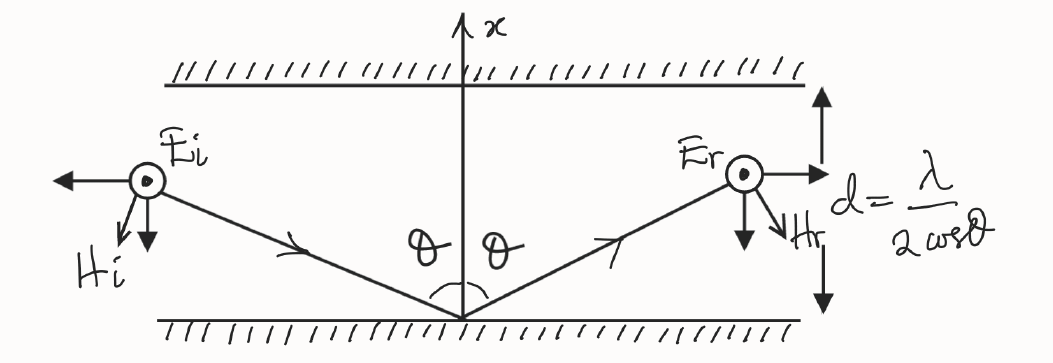
\includegraphics[width=1\linewidth]{\pathtoparttwo/graphics/lec35fig6}
\caption{Wave propagation in a parallel plane waveguide with distance set to $\frac{\lambda}{2\cos\theta}$}
\label{fig:lec35fig6}
\end{figure}

\emph{Why does this happen?} The occurrence of discrete values for the mode parameter $m$ and its direct relation to the wave propagation behaviour within the waveguide can be understood from the physical properties of the waveguide structure itself.

Consider the case where $m=1$, and the distance between the two conducting planes is $d$. At $x=0$, we have $\sin(\frac{m\pi x}{d}) = \sin(\frac{\pi}{d})$. Since the sine function takes its first positive zero at $\frac{\pi}{2}$, we find that $\sin(\frac{\pi}{d})$ is zero at $x=\frac{d}{2}$. This means that the electric field experiences a half-cycle variation (from zero to maximum) within the distance from $x=0$ to $x=d$. This behaviour is illustrated in Figure~\ref{fig:lec35fig7} for $m=1$.

Similarly, for $m=2$, $\sin(\frac{m\pi x}{d})$ takes its first positive zero at $\frac{\pi}{d}$. Therefore, at $x=\frac{d}{2}$, we have $\sin(\frac{m\pi x}{d}) = \sin(\frac{2\pi}{d})$. Since the sine function has its first positive zero at $\pi$, we get $\sin(\frac{2\pi}{d})=0$ at $x=\frac{d}{2}$. This leads to a full cycle variation (from minimum to maximum and back to minimum) of the electric field within the distance from $x=0$ to $x=d$. The same pattern follows for $m=3$, where $\sin(\frac{m\pi x}{d})$ takes its first positive zero at $\frac{\pi}{d}$ and the second positive zero at $\frac{2\pi}{d}$, resulting in $1\frac{1}{2}$ cycle variations of the electric field within the distance from $x=0$ to $x=d$.
\begin{figure}[h]
\centering
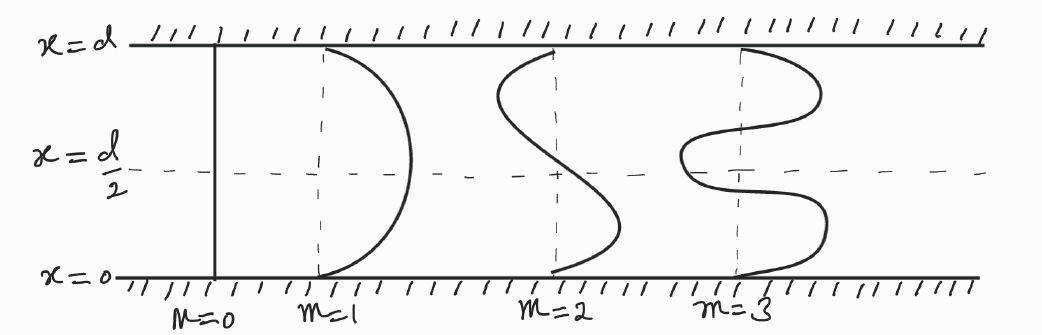
\includegraphics[width=1\linewidth]{\pathtoparttwo/graphics/lec35fig7}
\caption{Electric Field variation with different values of $m$}
\label{fig:lec35fig7}
\end{figure}

So the mode parameter, `$m$', signifies the number of half-cycle variations of the electric field (or magnetic field) amplitude that occur in the direction transverse to the net wave propagation. For instance, when $m=0$, the electric field remains constant along the transverse direction. Consequently, to satisfy the boundary conditions at the conducting planes, the electric field must be zero everywhere. As a result, the $m=0$ mode is physically impossible inside the waveguide, and no wave can propagate in this mode. That is what the bold part of the expression, $\bar{E} = \jmath 2E_i\boldsymbol{\sin(\frac{m\pi x}{d})}e^{-\jmath 2\beta\sqrt{1 - \left(\frac{m\lambda}{2d}\right)^2}}$, signifies.

However, the lowest value of $m$ that can propagate within the structure is $m=1$, also known as the `TE$_1$' mode. In this mode, there is one half-cycle variation of the electric field amplitude in the direction transverse to the propagation direction. This variation allows the electric field to be zero at both conducting boundaries, thereby fulfilling the boundary conditions and enabling sustained wave propagation along the waveguide.

For higher values of $m$ (e.g., $m=2$, $3$, and so on), the mode exhibits multiple half-cycle variations in the transverse direction, leading to more complex field distribution patterns with multiple peaks and nulls.

It is important to note that the value of $m$ depends on the spacing of the conducting planes and the specific mode of operation. Only certain discrete values of $m$ support sustained propagation within the waveguide, resulting in a quantized and discrete nature of modes. These distinct modes, such as `TE$_1$', `TE$_2$', `TE$_3$', etc., each possess unique field patterns and specific angles of incidence that facilitate their propagation within the waveguide. This discrete nature of modes is fundamental to waveguides' functioning and has significant implications for their performance and design considerations.

\begin{exmp}
\subsubsection*{Electric and Magnetic fields in a Parallel Plate Waveguide}
An air-filled parallel plane waveguide has a 10cm separation between the plates. The maximum peak electric field is 100V/m. If the frequency of operation is 10GHz, and if the waveguide is excited in the `TE$_1$' mode, find the expressions of the electric and magnetic fields inside the waveguide.

\subsubsection*{Solution}
The separation between the plates is $d = 10cm = 0.1m$. The frequency of operation is $f = 10GHz = 10\times 10^9Hz$. The maximum peak electric field is $E_i = 100V/m$. The waveguide is excited in `TE$_1$' mode, so $m=1$.

Assuming the wave propagates in the z-direction and the electric field points in the y-direction then from Equation~\eqref{eqn:totalelectricfield3}, we have
\begin{align*}
\bar{E} = \jmath 2E_i\sin(\frac{m\pi x}{d})e^{-\jmath 2\beta z\sqrt{1 - \left(\frac{m\lambda}{2d}\right)^2}}\hat{y}
\end{align*}
Let us find the wavelength, $\lambda$ and the phase constant, $\beta$.
\begin{align*}
\lambda &= \frac{c}{f}\quad\text{where } c = 3\times 10^8m/s\\
&= \frac{3\times 10^8}{10\times 10^9}\\
&= 0.03m
\end{align*}
\begin{align*}
\beta &= \frac{2\pi}{\lambda}\\
&= \frac{2\pi}{0.03}\\
&= 200\pi
\end{align*}
Thus,
\begin{align*}
\bar{E} &= \jmath 2\times100\sin(\frac{m\pi x}{d})e^{-\jmath 2\times200\pi z\sqrt{1 - \left(\frac{m\lambda}{2d}\right)^2}}\hat{y}\\
&= \jmath 200\sin(\frac{\pi x}{0.1})e^{-\jmath 400\pi z\sqrt{1 - \left(\frac{\lambda}{0.2}\right)^2}}\hat{y}\\
&= \jmath 200\sin(10\pi x)e^{-\jmath 400\pi z\sqrt{1 - {(5\lambda)}^2}}\hat{y}\\
&= \jmath 200\sin(10\pi x)e^{-\jmath 400\pi z\sqrt{1 - {(5\times0.03)}^2}}\hat{y}\\
&= \jmath 200\sin(10\pi x)e^{-\jmath 400\pi z\sqrt{0.7975}}\hat{y}\\
&= \jmath 200\sin(10\pi x)e^{-\jmath 356.8\pi z}\hat{y}\quad V/m
\end{align*}

For the magnetic field, we have two components, $H_x$ and $H_y$, so from Equations~\eqref{eqn:totalmagfieldx4} and \eqref{eqn:totalmagfieldz3}, we have
\begin{dmath*}
\bar{H} = j2\frac{E_i}{\eta}\sin\theta\sin(\frac{m\pi x}{d})e^{-j2\beta z\sqrt{1 - \left(\frac{m\lambda}{2d}\right)^2}}\hat{x} - 2\frac{E_i}{\eta}\cos\theta\cos(\frac{m\pi x}{d})e^{-j2\beta z\sqrt{1 - \left(\frac{m\lambda}{2d}\right)^2}}\hat{z}
= 2\frac{E_i}{\eta}\left\{j\sin\theta\sin(\frac{m\pi x}{d})\hat{x} - \cos\theta\cos(\frac{m\pi x}{d})\hat{z}\right\}e^{-j2\beta z\sqrt{1 - \left(\frac{m\lambda}{2d}\right)^2}}
= 2\times\frac{100}{377}\left\{j\sin\theta\sin(\frac{\pi x}{0.1})\hat{x} - \cos\theta\cos(\frac{\pi x}{0.1})\hat{z}\right\}e^{-j2\beta z\sqrt{1 - \left(\frac{\lambda}{0.2}\right)^2}}
= 0.5305\left\{j\sqrt{1 - \left(\frac{m\lambda}{2d}\right)^2}\sin(10\pi x)\hat{x} - \frac{m\lambda}{2d}\cos(10\pi x)\hat{z}\right\}e^{-j2\times200\pi z\sqrt{1-\left(\frac{0.03}{0.2}\right)^2}}
= 0.5305\left\{j\sqrt{1-\left(\frac{0.03}{0.2}\right)^2}\sin(10\pi x)\hat{x} - \frac{0.03}{0.2}\cos(10\pi x)\hat{z}\right\}e^{-j2\times200\pi\times 0.9887 z}
= 0.5305(j0.9887\sin(10\pi x)\hat{x} - 0.15\sin(10\pi x)\hat{z})e^{-j356.8z} H/m
\end{dmath*}
The field components of the wave propagating at 10 GHz have been calculated.
\end{exmp}

\section{Trough of a mode}\index{Trough of a mode}
On a given structure, we can have multiple modes propagating depending upon how the angles $\cos\theta = \frac{m\lambda}{2d}$ can be satisfied. $m=1$ is the lowest mode, so the question is \emph{what wave can survive in mode 1?} With $\cos\theta = 1$, $\dfrac{m\lambda}{2d} = 1$, hence, $\lambda = 2d$ or $d = \dfrac{\lambda}{2}$. This implies that the separation between the planes is $\dfrac{\lambda}{2}$. Thus in TE$_1$ mode the smallest separation is $\dfrac{\lambda}{2}$, if it is less than $\dfrac{\lambda}{2}$, we cannot have an angle as $\dfrac{m\lambda}{2(0.4\lambda \text{ assume})}> 1$, so that $cos\theta > 1$. No physical angle has its cosine greater than 1. So the lowest mode for which the wave can propagate in the structure has $d \geq \dfrac{\lambda}{2}$\footnote{
This makes $cos\theta \leq 1$
}. So not only that the separation distance $d$ is given, but a wavelength is required for which $d\geq\dfrac{\lambda}{2}$ or inverted $\lambda \leq 2d$. This means the frequency has to be above certain values so that $\lambda \leq 2d$ is satisfied, only then will the wave propagation take place. If $\lambda > 2d$ or frequency is less than certain values, then wave propagation cannot take place inside the structure.

With this, we get an important concept of what is called the \textbf{Trough} of a mode, that is when $d = \dfrac{\lambda}{2}$ or $\lambda = 2d$ which is the lowest frequency that can propagate on a waveguide whose separation is $d$.
\begin{dmath}
\lambda_\max = 2d
\label{eqn:cut-offlambda}
\end{dmath}
\begin{dmath*}
\frac{c}{f_\min} = 2d
\end{dmath*}
\begin{dmath}
f_\min = \frac{c}{2d}
\label{eqn:cut-offf}
\end{dmath}
Equations~\ref{eqn:cut-offlambda} and \ref{eqn:cut-offf} are the maximum wavelength and minimum frequency respectively that define wave propagation. Below $f_\min$, the wave doesn't propagate and that is the minimum frequency for $m=1$ mode and it is called the cut-off frequency of that mode. So for a particular mode to propagate the frequency must be above that value and that is called the cut-off frequency for that mode.

The cut-off frequency is the lowest frequency that would propagate inside the structure for a given mode number or given $m$. Either we see that or the mode increases to TE$_2$, the frequency will be doubled and so on. Hence the reason we say the lowest mode is because that is the lowest frequency in the structure which can propagate.

Substituting $d=\dfrac{\lambda}{2}$ and $m=1$ in equation ~\ref{eqn:phaseconst} gives:
\begin{dmath*}
\bar{\beta} = \beta\sqrt{1 - \left(\frac{m\lambda}{2d}\right)^2} =  \beta\sqrt{1 - \left(\frac{\lambda}{2\left(\frac{\lambda}{2}\right)}\right)^2} = 0
\end{dmath*}
This shows that the frequency at $d=\dfrac{\lambda}{2}$ which is the cut-off frequency, the phase constant of the wave goes to zero. Below this frequency $\left(\dfrac{m\lambda}{2d}\right)^2 > 1$, the expression $\sqrt{1 - \left(\frac{m\lambda}{2d}\right)^2}$ in the phase constant is imaginary, so $\bar{\beta}$ becomes imaginary. It is no more a phase constant but becomes an attenuation constant i.e. the wave losses its wave nature in the presence of a field that is dying down exponentially. So below the cut-off frequency, it represents a field that is exponentially decaying and hence no propagation of electromagnetic waves.

What we see from this analysis is that when we have a band structure like a parallel plane waveguide, first there are the discrete angles at which uniform plane waves are bouncing back and forth between two parallel planes giving the field distribution and those field patterns we call modal patterns. We also see that for a given mode number, the frequency has to be above certain values called cut-off frequency for that mode. So depending on the mode you want to excite, you require a certain frequency. So even if the waveguide is capable of supporting the different values of $m$, it would depend on the frequency whether the wave will be accepted or not i.e. if the frequency is greater than the cut-off frequency or not. This is the basic picture of modal propagation within a bounded structure like a waveguide. We will elaborate on this and then following this, we will try to see other modes and then move on to complex structures like the rectangular waveguides.

\section*{Exercises}
\begin{ExerciseList}
\Exercise[label={ex351}]
Starting with a diagram and basic field expressions show that the distance between conducting boundaries in a parallel plane waveguide is given by $d = \frac{m\pi}{\beta\cos\theta}$ when m is an integer and $\theta$ is the angle of incidence.
\Exercise[label={ex352}]
From the developed expressions in Ex.~\ref{ex352}, derive a formula that shows with the aid of a graph that the parameter m indicates the number of half-cycle amplitude variations across the distance between the conducting planes.
\Exercise[label={ex353}]
Given that a  5 GHz wave is launched at an angle of 60\textdegree into an air-filled parallel-plate waveguide operating in TE mode calculates the phase constant.
\Answer[ref={ex353}]
90.69rad/m
\Exercise[label={ex354}]
If a 50 GHz wave is launched into a parallel plane waveguide that has a separation of 1cm between the planes, calculate the largest possible launch angle (but less than 90\textdegree) required for the wave to propagate.
\Answer[ref={ex354}]
72.51\textdegree

\end{ExerciseList}
